%%%%%%%%%%%%%%%%%%%%%%%%%%%%%%%%%%%%%%%%%%%%%%%%%%%%%%%%%%%%%%%%%%%%%%%%%%%%%%%%%%%%%
% Template revision history:
% BS02022: Revised by Sukumar Natarajan, s.natarajan@bath.ac.uk
% BS2021: Revised by Filip Jorissen, filip.jorissen@kuleuven.be
% BS2019: Revised by Alessandro Prada, alessandro.prada@unitn.it
% BS2017: Initial version by Michael Wetter, mwetter@lbl.gov
%%%%%%%%%%%%%%%%%%%%%%%%%%%%%%%%%%%%%%%%%%%%%%%%%%%%%%%%%%%%%%%%%%%%%%%%%%%%%%%%%%%%%

\documentclass[twocolumn, a4paper,10pt]{article}
\usepackage[top=2.5cm, bottom=2.5cm, left=2.0cm, right=2.0cm,
columnsep=0.8cm]{geometry}
\usepackage{enumitem}
\usepackage[hidelinks]{hyperref}
\usepackage{boxedminipage}
\usepackage{nopageno}
\usepackage{graphicx}
\usepackage{natbib}
\usepackage[font=it]{caption}
\usepackage[usenames,dvipsnames]{xcolor}
\usepackage{listings}
\usepackage{float}
\usepackage{amsmath}
\usepackage{caption}
\usepackage{subcaption}
%-----------------------------SET SKIP SPACES -------------------------------------------------------------------
\setlength{\abovecaptionskip}{0pt}
\setlength{\belowcaptionskip}{3pt}
\setlength{\parindent}{0pt}
\setlength{\parskip}{3pt}
%\renewcommand{\baselinestretch}{0.7}
% FOR enumerates
\setlist{itemsep=-0.1cm,topsep=0.1cm,labelsep=0.3cm}
\setenumerate{leftmargin=*}
\setcounter{secnumdepth}{-1}
%-----------------------------SET FONTS -------------------------------------------------------------------
% Set fonts for title, section and subsection headings
\makeatletter
\renewcommand\title[1]{\gdef\@title{\fontsize{12pt}{2pt}\bfseries{#1}}}
\makeatletter
\renewcommand\section{\@startsection{section}{1}{\z@}{3pt}{3pt}{\normalfont\large\bfseries}}
% \normalfont\large
\makeatletter
\renewcommand\subsection{\@startsection{subsection}{1}{\z@}{\z@}{\z@}{\normalfont\normalsize\bfseries}}
\makeatletter
\renewcommand\subsection{\@startsection{subsection}{1}{\z@}{\z@}{0.1pt}{\normalfont\normalsize\bfseries}}
\renewcommand\refname{References}
%END OF THE SETUP
%%%%%%%%%%%%%%%%%%%%%%%%%%%%%%%%%%%%%%%%%%%%%%%%%%%%%%%%%%%%

%%%%%%%%%%%%%%%%%%%%%%%%   TITLE   %%%%%%%%%%%%%%%%%%%%%%%%%%%%%%%
%%% Please keep the \vspace{4pt} at the top
\title{%
RoofKIT – Building simulation in sustainable housing at \\% Line 1
%%% Please keep the \vspace{4pt} between lines in the title
\vspace{4pt}
the Solar Decathlon Europe 21/22} % Line 2 
%If there is no second line then just put \phantom{Line 2} here
%%% Change or delete text before "\\" on the lines below to keep the layout but don't remove the "\\"
%%% Do not exceed more than 6 lines for authors and affiliations
\author{% Line 3
Nicolas Carbonare$^1$, Moritz Bühler$^2$, Jens Pfafferott$^2$, Andreas Wagner$^1$\\ % Line 4
$^1$Building physics group, Karlsruhe Institute for Technology, Karlsruhe, Germany\\ % Line 5
$^2$Institute of Sustainable Energy Systems, Offenburg University of Applied Sciences,\\% Line 6
Offenburg, Germany\\ % Line 7
\phantom{Line 8}\\ % Line 8
\phantom{Line 9}\\} % Line 9
\date{\vspace{-0.5cm}}	% remove default date and replace the Blank 10th line														% Line 10
%END OF THE TITLE
%%%%%%%%%%%%%%%%%%%%%%%%%%%%%%%%%%%%%%%%%%%%%%%%%%%%%%%%%%%%
\begin{document}

\maketitle
\section*{Abstract}	% Section headings need to be upper and lower case.
\addtocounter{section}{1}
The contribution of the RoofKIT student team to the SDE 21/22 competition is the extension for an existing café in Wuppertal, Germany, to create new functions and living space for the building with simultaneous energetic upgrading. A demonstration unit is built representing a small cut-out of this extension. The developed energy concept was thoroughly simulated by the student team in seminars using Modelica. The system uses mainly solar energy via PVT collectors to as the heat source for a brine-water heat pump (space heating and hot water). Energy storage (thermal and electrical) is installed to decouple generation and consumption. Simulation results confirm that carbon neutrality is achieved for the building operation, consuming and generating around 60 kWh/$m^2$a.

\section*{Key Innovations}
\begin{itemize}
\item Building and system simulation in educational context
\item Simulation-based decision-making in real building design
\item Students from different background and professionals together to achieve an overall concept for simulation-aided design
\end{itemize}

\section*{Practical Implications}
This publication highlights the relevance of including building performance simulation as part of the design process in an educational context for architects and engineers. Throughout the entire duration of the project, the simulation work was carried out by students of different degrees and universities, ensuring a dissemination of the relevance of building simulation. A successful knowledge transfer will widen the implementation of simulation-based decision making in the forthcoming years, and therefore accelerate the path to the climate targets in 2050.  

\section*{Introduction}
The U.S. Department of Energy\textsuperscript{\textregistered} Solar Decathlon is a student competition that began in 2002. The ten contests challenge students to design and build low-energy buildings that mitigate climate change and improve indoor environmental quality through greater affordability, resilience, energy efficiency and comfort. The teams must blend architectural and engineering excellence with innovation at its best. The expansion of the solar decathlon to its European (SDE) version started in 2010, and being held in 2021/2022 for the fifth time in Wuppertal, Germany (see \textcolor{blue}{\url{https://sde21.eu/}}).\\
Within the scope of this competition, student teams from all over the world must design, build and operate experimental houses. For the 21/22 edition, these houses are built in the so-called "Solar Campus" in Wuppertal (Figure \ref{fig:SDE}). To make the assembly, disassembly and transportation process possible, the houses are small, lightweight construction, with a high degree of prefabrication. The SDE rules have a juried and monitored contests. For the European editions, around 40\% of the maximum 1000 points are distributed based on monitoring results at the solar campus, concerning energy performance and indoor environmental quality. More about the contests can be found in the literature (\citet{voss2021}).

\begin{figure}[H]
\centering
\includegraphics[trim={0cm 10cm 17cm 6cm}, clip, scale=0.11]{img/RoofKIT-01-©-SDE-2021-22-scaled.jpg}
\vspace{2pt} 
\caption{Overview of the Solar Decathlon Europe 21/22.\copyright SDE 21/22}
\label{fig:SDE}
\end{figure}
\vspace{-2pt}

In all European competitions, the teams must provide simulation results to proof the year-round suitability of the energy concepts as part of the requirements. The goal is to guarantee a dissemination of building simulation as a powerful tool to provide energy-efficient and innovative solutions in buildings. Besides, this helps to ensure the usability of the houses during the whole year. \\
The student team RoofKIT of the Karlsruhe Institute of Technology (KIT) participated for the first time at the SDE 21/22, obtaining the first place in the overall ranking. In view of the advancing climate change as well as the shrinking natural material resources, the team believes fundamental rethinking in building industry is necessary. The further development and conversion of the existing building stock, circular design and urban mining, the use of environmental-friendly materials as well as a CO2-neutral energy supply are core tasks of the construction sector. This contribution describes part of the building simulation challenges that the team performed for the competition, not only as part of the required tasks, but also to support the decision-making process of the proposed integral design.

%---------------------------------------------------------------------------------------
\section*{The RoofKIT project}
%---------------------------------------------------------------------------------------
Seeking for innovative strategies for the densification and revitalization of the existing European city, the RoofKIT team worked on the extension of the Café ADA in the Mirker district of Wuppertal, Germany. RoofKIT not only creates new living space, but takes the historic building as the initial point for an integrated solar-based design concept. The exterior of the existing building remains largely unchanged to remain as a point of identification in the neighborhood, with an energetic upgrade of the building envelope, without neglecting the indoor environmental quality. A newly designed ballroom was moved up one floor. Through its form and materiality, it spatially forms a transition between the existing building and the new structure. The additional residential units on top of the new ballroom are manufactured as prefabricated wooden modules. This allows for quick and simplified assembly on the construction site. The elevation presents a concept of shared spaces to renegotiate available individual as well as commonly used space. Thus, RoofKIT aims to address the needs of residents in different living situations, among them students, families and seniors, and shall help to create a social togetherness.\\
For the competition in Wuppertal, a residential unit from the elevation was simplified and "cut out" as a demonstrator - the House Demonstration Unit (HDU). Despite being a part of the whole building, the HDU had specific requirements but also offers opportunities, e.g. it does not build up on an existing building and it has a better ratio between available solar envelope and conditioned volume. As a construction, it consists of four prefabricated modules with a central core that bundles all technical installations as well as the kitchen and bathroom. This leaves almost the entire net floor area of the unit (54 $m^2$) free for living, working and sleeping. To demonstrate the elevation, the building unit was placed on scaffolding, and the area underneath the building was additionally used during the competition for visitor access, in allusion to the dance hall, but also for technical equipment that would otherwise be found in technical rooms in the existing building. Figure \ref{fig:HDU} shows a picture of the HDU during competition in Wuppertal. The HDU will be further used as a guest house at KIT in Karlsruhe in the near future. More information about the project and the building design can be found on the building competition (\textcolor{blue}{\url{https://building-competition.org/EU2021/KIT/}}) and the project website (\textcolor{blue}{\url{https://roofkit.de/en/}}).

\vspace{-2pt} 
\begin{figure}[H]
\centering
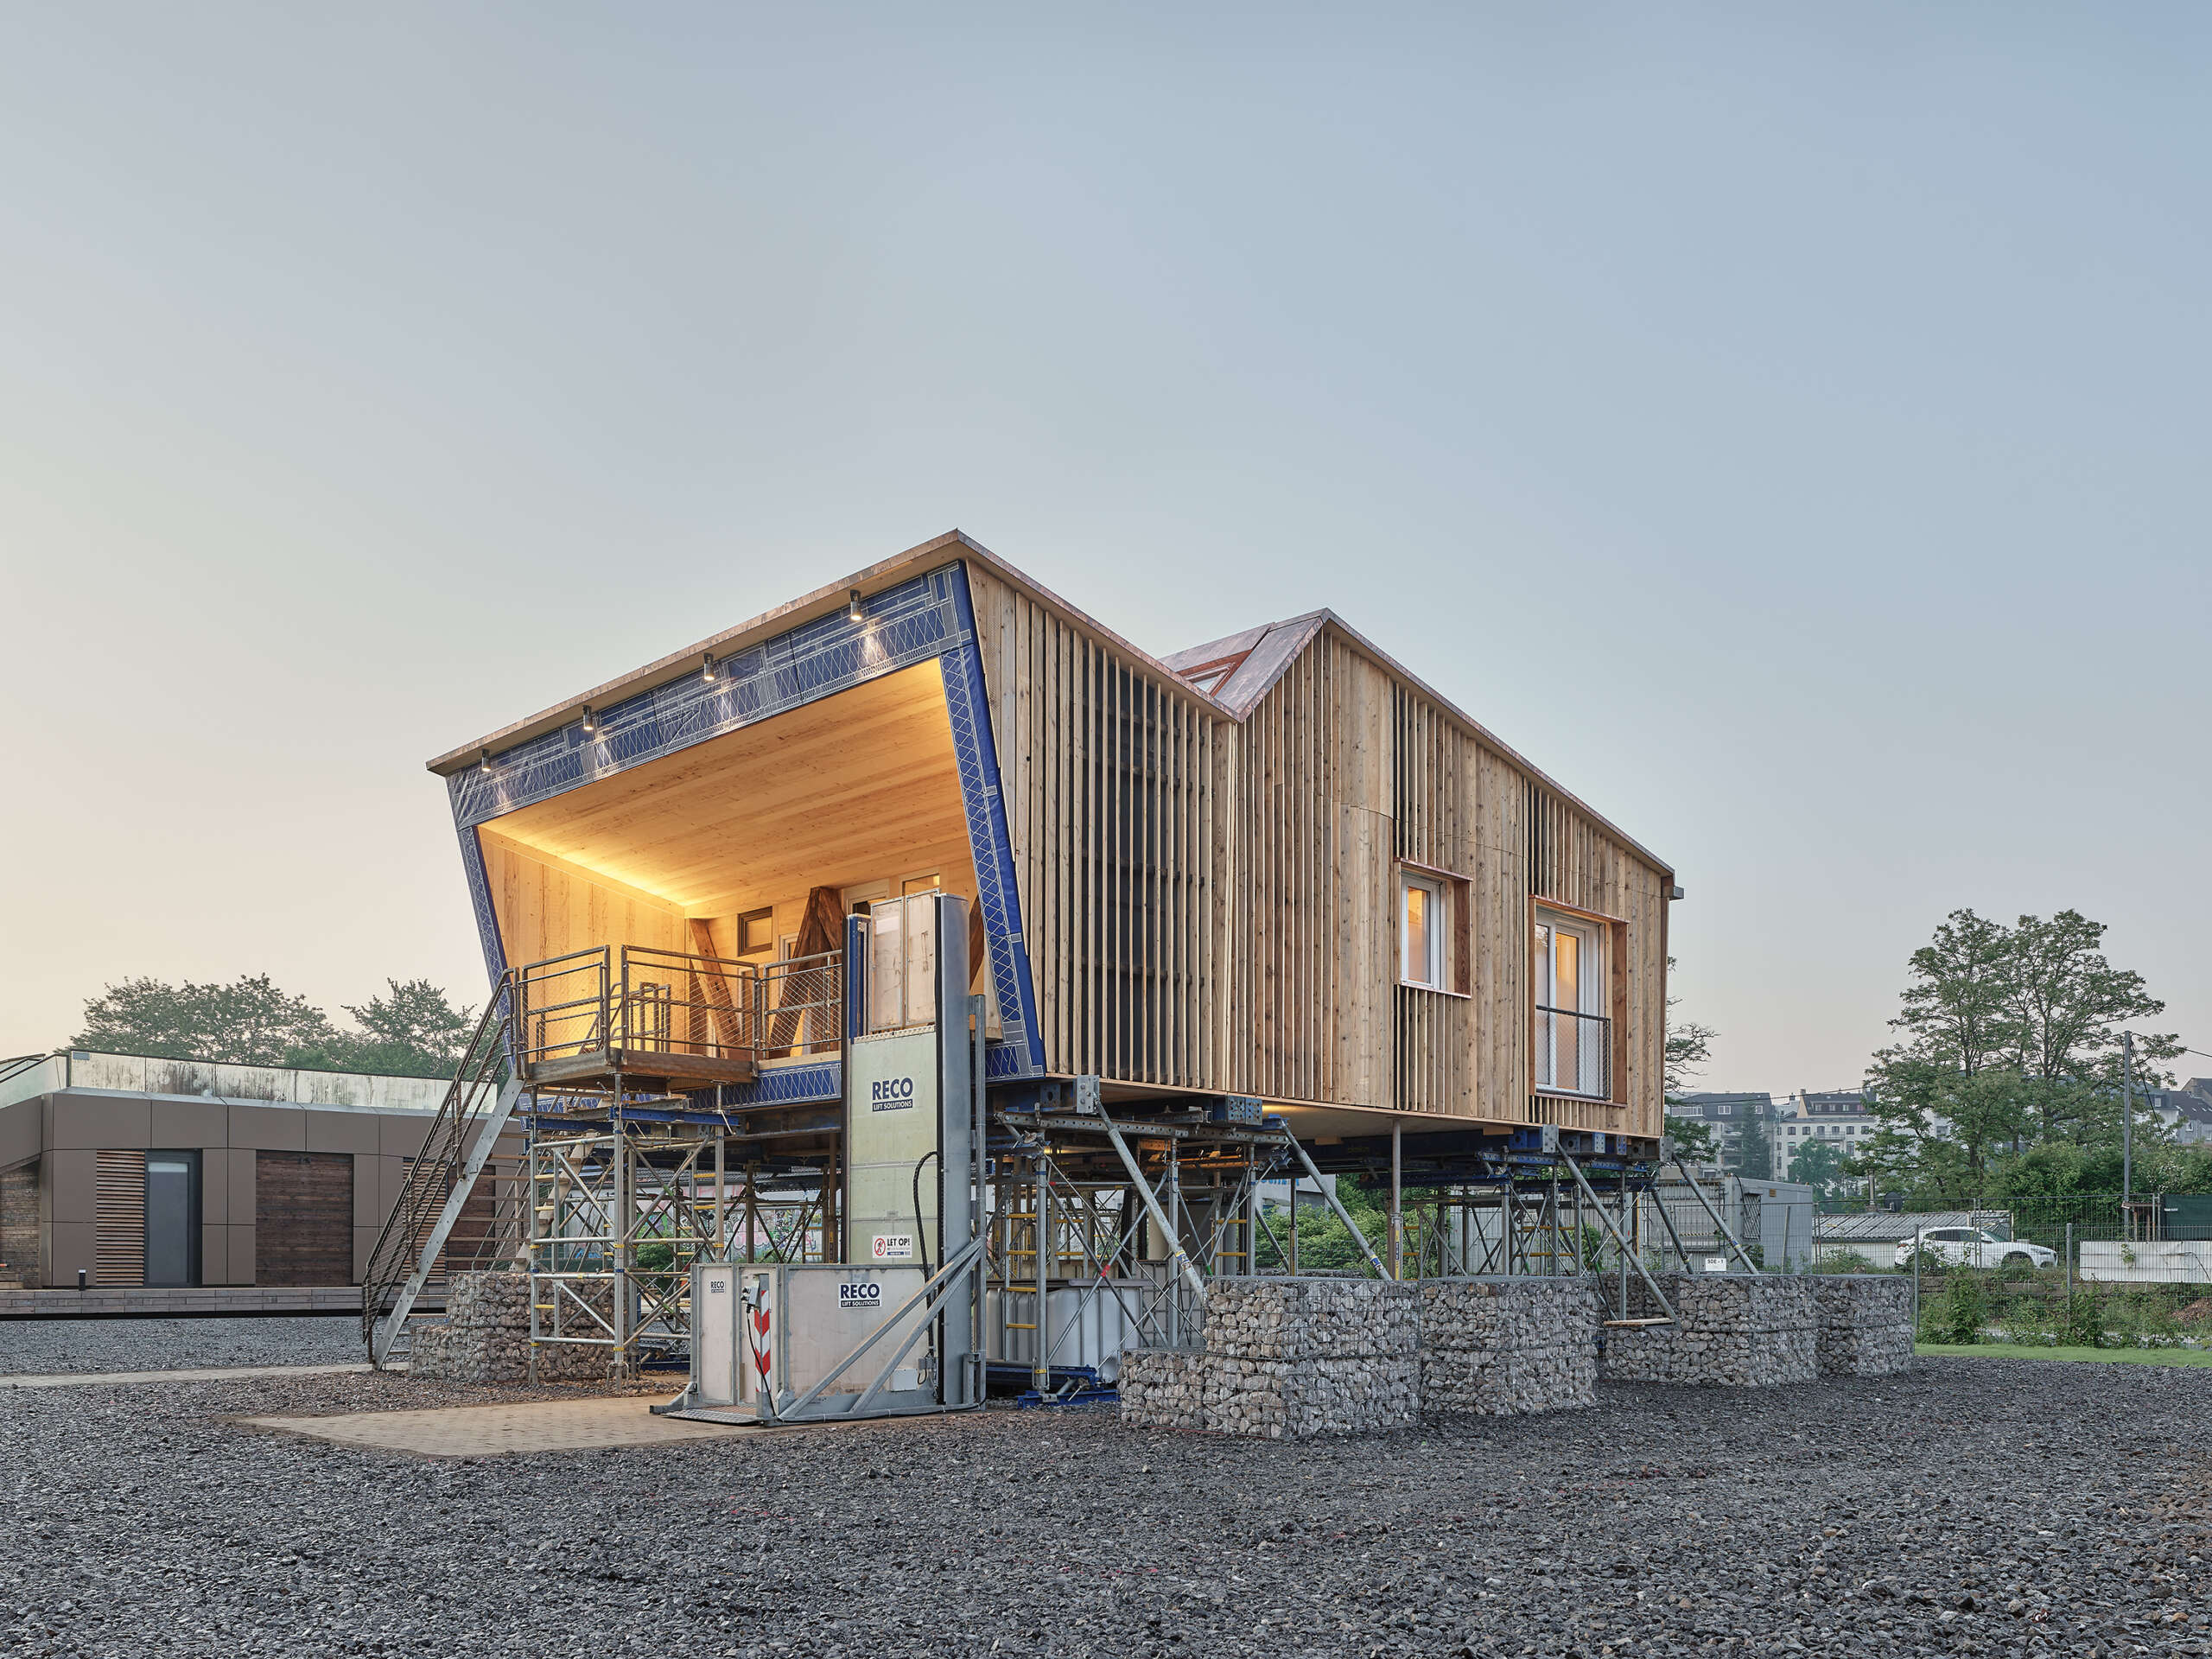
\includegraphics[trim={8cm 4cm 10cm 12cm}, clip, scale=0.11]{img/Zooey-Braun701-01-1-scaled.jpg}
\vspace{2pt} 
\caption{View of the House Demonstration Unit during competition.\copyright Zooey Braun}
\label{fig:HDU}
\end{figure}
\vspace{-2pt} 

%---------------------------------------------------------------------------------------
\subsection*{Building envelope}
%---------------------------------------------------------------------------------------
Wood from various recycled stages was used for the load-bearing structure of the HDU as well as for sheathing to further reduce the global warming potential of the building also through stored CO2. In addition, the reuse of all materials and components was ensured through mono-fraction construction without non-detachable connections as far as possible. The thermal insulation of the entire building envelope was realized with a natural product based on seaweed, which is processed into insulating material without additives and offers good thermal properties in comparison to conventional insulation materials. Since the HDU is elevated and thus connects to outside air on all six sides, the floor area must also meet the high requirements for thermal insulation - unlike in the case of an extension.\\
Another special feature of the HDU are the windows; here so-called stock windows, i.e. windows from or for other construction projects, are used for the HDU. The primary selection criterion was adequate thermal insulation; different window sizes are used as a design feature. The glazing with a solar transmission of 0,59 still allows for solar gains in winter but requires a very effective solar protection system for summer conditions.\\
Additional thermal mass was implemented into the lightweight construction to guarantee successful passive cooling and achieve comfortable indoor spaces in summer. Clay boards were integrated into the inner wall surfaces (together with loam rendering) as well as in two layers in the floor (above and in good contact with the floor heating pipes). Besides their outstanding performance regarding heat buffering, clay is an excellent moisture buffer as well. For effectively discharging the thermal mass by night ventilation, reasonable ventilation rates must be achieved. Decentralized mechanical ventilation units can achieve around 0,8 ACH at nominal speed, whereas natural ventilation was designed to provide air exchange rates between 4 and 6 ACH. Therefore, a night ventilation concept with the windows and a skylight in the bathroom area was implemented. Thus, the buoyancy effect can be utilized, guaranteeing higher air change rates with air entering through the windows and exhausting through the skylight.  Table \ref{tab:properties} shows a summary of the building's thermal properties.\\

\begin{table}[ht]
\vspace{-5pt}   % Please use appropriate negative vspace to remove the space above/below the Table
\caption{Building thermal properties.}
\label{tab:properties}
\centering
\begin{tabular}{| c | c | c | }
  \hline
  \bf{Indicator} & \bf{Unit} & \bf{Value} \\
  \hline
  U-value exterior wall & W/$m^2$K & 0.20 \\
  U-value ceiling & W/$m^2$K & 0.14 \\
  U-value floor & W/$m^2$K & 0.18 \\
  U-value windows & W/$m^2$K & 0.6 \\
  g-value windows & - & 0.59 \\  
  Specific thermal mass & $Wh/m^{2}k$ & 76.0 \\
  Infiltration rate $n_{50}$ & $h^{-1}$ & 0.5 \\
  \hline
\end{tabular}
\vspace{-5pt}   % Please use appropriate negative vspace to remove the space above/below the Table
\end{table}

%---------------------------------------------------------------------------------------
\subsection*{Energy concept}
%---------------------------------------------------------------------------------------
Figure \ref{fig:HDU_SimConcept} illustrates the scaled-down solar energy supply concept, that was adapted to the requirements of the small building unit. Despite the fact that the HDU's south oriented sloped roof would offer enough space for separate thermal and photovoltaic collectors, the idea of efficient double use of this space with PVT collectors was adopted from the whole building approach to demonstrate a general solution for extensions in urban situations.\\ 
A heat pump (with a nominal heating capacity of 6 kW) provides domestic hot water and heating energy supply for the HDU. The heat pump has an integrated tank for domestic hot water (185 l) with an electric heater as a backup. The piping system for hot water is made of copper. A floor heating system provides thermal comfort in winter. The heat pump comes with an integrated modulating control strategy, that allows a direct integration of the heat pump into the floor heating circuit, therefore disregarding a buffer tank on the sink side of the system.\\
The roof is covered with 18 solar modules in total (29 $m^2$). Simulations showed that 12 PVT collectors are enough to serve as a heat source for the heat pump. The modules are connected in parallel on the thermal side to reach the required mass flow through the collector field. A buffer storage of 1000 l separates the brine-filled collector circuit and the heat pump's evaporator circuit and helps to adapt the operation of the collectors to periods with sunshine and ambient temperatures above 0°C to avoid icing around their fluid pipes. This system design was a consequence of the architectural decision to apply flat roof-integrated PVT-collectors to have an aesthetically well-integrated system.\\
In addition to the 12 PVT-collectors, 6 more PV modules are installed to reach a homogeneous roof cover and to provide enough electricity for the later operation of the HDU in Karlsruhe (heat pump, household electricity, mobility) on an annual basis. The PV modules have a rusty brown color which is identical to the roof color – as an additional an architectural integration measure. Applying an innovative coating technique, the PV modules show a comparably high efficiency (18\% reported by the company). Generally, PVT technology helps to increase PV output as the solar cells are cooled by the brine circuit. For the SDE competition in Wuppertal, only 10 PV modules were connected to the electrical system to not exceed the limit for PV output of 3kWp, given by the SDE rules. The inverter and battery (limited to 2.5 kWh by the competition) are installed below the building.\\
The energy consumption of the HDU is optimized by an energy management system, with a particular focus on energy efficiency and self-consumption. The following components are used as actively controllable components in the HDU: The battery, the heat pump, the decentralized ventilation systems, the skylights, the shading systems of the windows and a controllable socket to which an e-bike can be connected for charging. Besides, a weather station is installed on the roof to capture all necessary weather data locally, and also two indoor environmental sensors (room temperature, relative humidity and CO2 concentration) are installed on both sides of the HDU. All components are connected to the energy management system using an open source software BEMCom (\citeyear{Woelfle2022}).

\begin{figure*}[ht]
\centering
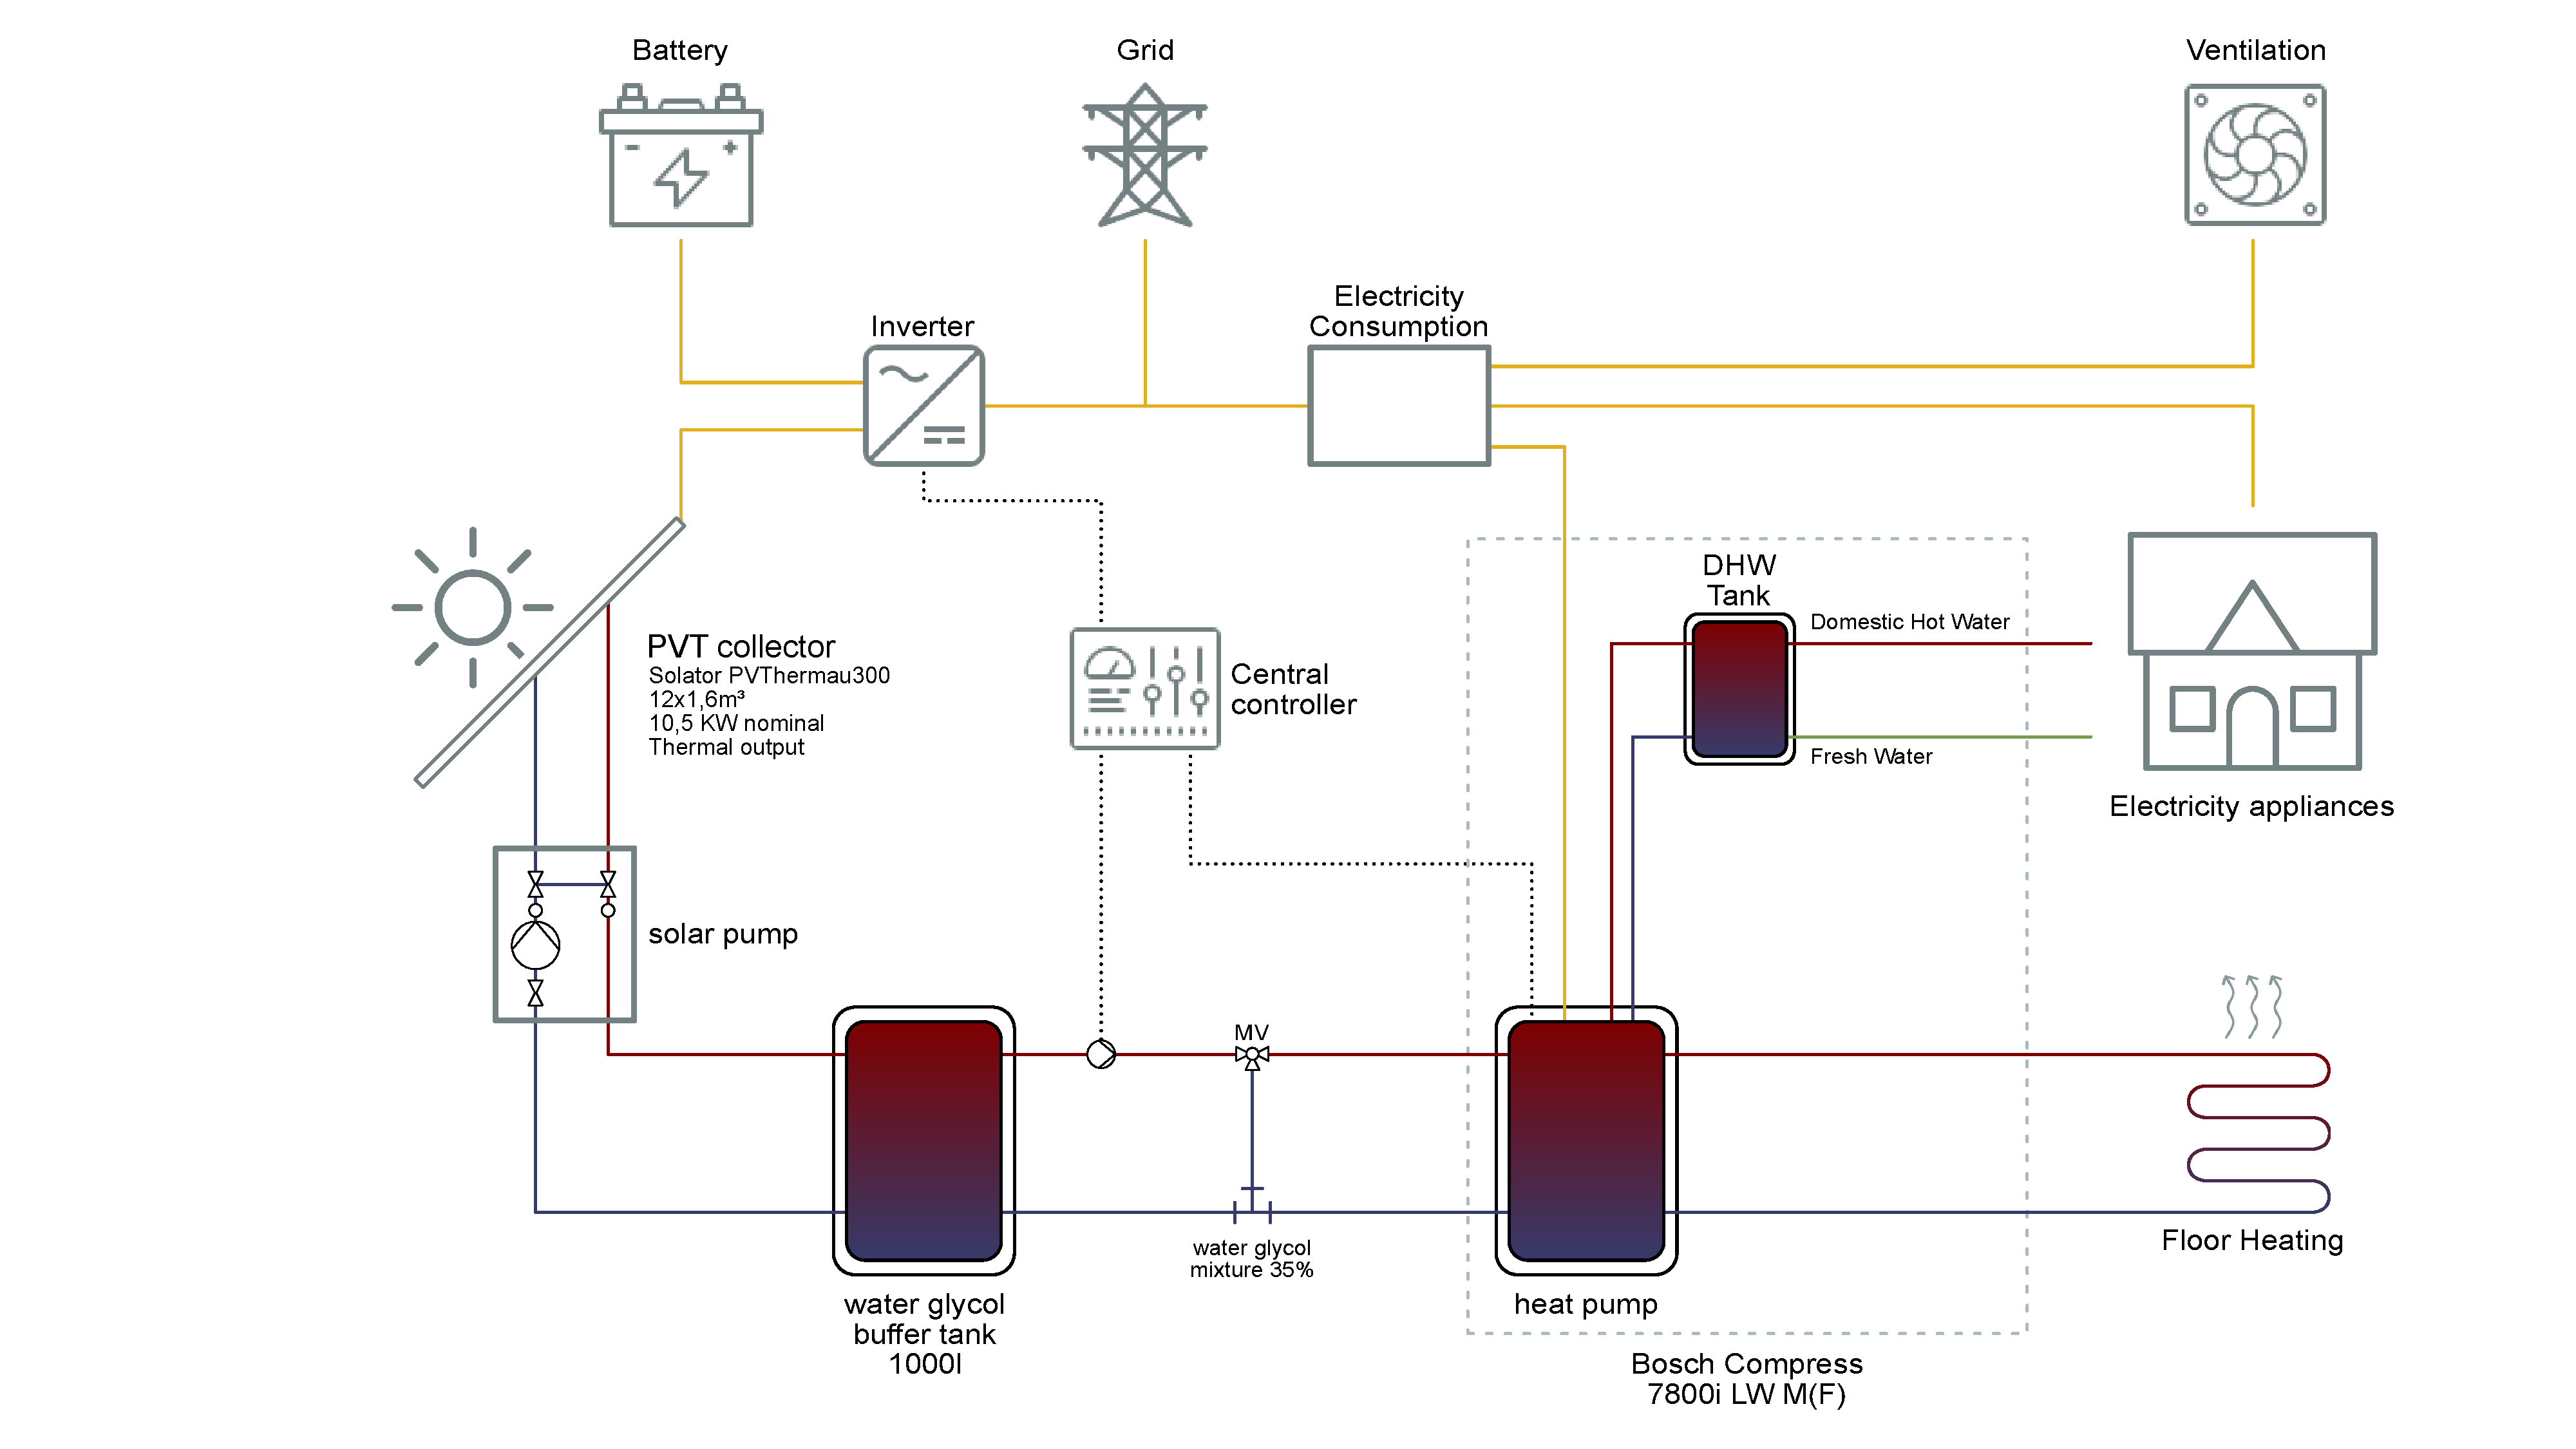
\includegraphics[trim={9cm 0 0 0},scale=0.3]{img/HDU_SimConcept.pdf}
\vspace{-5pt} 
\caption{Schematic diagram of the energy concept of the House Demonstration Unit - simulated in Modelica.}
\label{fig:HDU_SimConcept}
\end{figure*}

%---------------------------------------------------------------------------------------
\section*{Model development}
%---------------------------------------------------------------------------------------
Extensive system simulations were performed to find the best possible design solution for the solar-based heating system. Many combinations with components (PVT collectors, buffer and domestic hot water tanks, heat pump) and their hydraulic connections were investigated, including a sensitivity analysis regarding the number of PVT collectors, to maximize the use of solar energy over the year and to minimize CO2 emissions from operating the system with electricity from the grid. Several control strategies (battery charging, heat pump, floor heating and solar water heating system) were developed to optimize the system behavior using these simulations. The system simulation was carried out in OpenModelica \citet{Fritzson2006} with hourly time steps. The model for the whole system was developed from the system design and parameterized according to the components' specifics. The weather file of Düsseldorf (due to its proximity to Wuppertal) was applied for the simulations. The full simulation models and evaluation files are freely available on GitHub (\textcolor{blue}{\url{https://github.com/nicocarbo/RoofKIT}}).\\

%---------------------------------------------------------------------------------------
\subsection*{Building model}
%---------------------------------------------------------------------------------------
For the HDU, a simplified building energy model (5R1C model from the DIN EN ISO \citet{DIN13790}) was developed. This approach creates a thermal model of the HDU as a single air temperature node (with a certain heat capacity) and divides the heat flux into five categories: transmission losses (windows and walls), ventilation heat losses, internal loads, solar gains, and the resulting space heating load, depending on the selected temperature set point. Team RoofKIT followed this modelling approach to optimize the resulting U-values and thermal mass capacity values for the House Demonstration Unit, as well as taking care of the contruction details. The calibration of the building model was performed using the software SimRoom \citeyear {SimRoom2022}, and the results (space heating energy and indoor temperature) were transferred to the Modelica model. To perform this simulation, assumptions about the internal loads (2-person household, 150 l hot water consumption per day, 1200 kWh electricity per person) and ventilation losses ($n_{50}$ = 0.5 $h^{-1}$) were defined. Electricity load profiles were obtained from the BDEW standard profiles (\citet{BDEW2002}). For the ventilation systems, a constant fan speed of 33\% was assumed during the whole year. The mobility electricity was calculated assuming a single E-bike that runs 8 km per day. Achieved air exchange rates during night ventilation in summer were estimated to be around 5 ACH, according to other simulation studies within this project. The results are available with the complete project documentation (\textcolor{blue}{\url{https://building-competition.org/EU2021/KIT/}}).\\

%---------------------------------------------------------------------------------------
\subsection*{Heating system and domestic hot water}
%---------------------------------------------------------------------------------------
The brine-water heat pump model was parameterized using a characteristic curve based on the inlet and outlet heat pump temperature (the influence of the mass flow rate was neglected, as both source and sink operate close to nominal volume flow with an on-off controller). The base model is the EquationFitReversible model from the Modelica Buildings Library (\cite{Wetter2014}). Equations \ref{eq:HPmodel} show the modelled behavior of the heat pump. 
\vspace{-5pt}

\begin{equation}
\begin{aligned}
\vspace{-3pt}
    &\dot{Q} = (\alpha1 + \alpha2 \frac{T_{loa,ent}}{T_{RefHeaLoa}} + \alpha3 \frac{T_{sou,ent}}{T_{RefHeaSou}}) \dot{Q}_0 \\
    &P= (\beta1 + \beta2 \frac{T_{loa,ent}}{T_{RefHeaLoa}} + \beta3 \frac{T_{sou,ent}}{T_{RefHeaSou}}) P_0
\label{eq:HPmodel}
\end{aligned}
\end{equation}

Domestic hot water and buffer storage tank were modeled with five layers to account for the stratification, including buoyancy effect between layers. The water tank model was used from the BuildingSystems library (\citet{NytschGeusen2012}). For the floor heating, all relevant physical parameters (to model the thermal inertia of the floor construction) for the different layers were implemented into the model. The floor heating is controlled using a heat curve from the heat pumps data sheet. Additionally, a hysteresis cycle for the heating temperature set point was included to avoid unstable system behavior.\\
According to the implemented control strategy, the PVT-collector loads the buffer tank. Hot water is then prepared with the heat pump, that operates at its highest possible efficiency in summer (COP = 5,85). The heat pump is capable of providing heat to the hot water tank and the floor heating at the same time. The controller to prioritize hot water or heating was developed for this simulation study. The daily domestic hot water usage is assumed 150 l at 43 °C (around 4 kWh per day) and the necessary maximum heating capacity for the HDU is 2 kW. Models for pumps valves and actuators were also taken from the Buildings library (\citet{Wetter2014}).\\

%---------------------------------------------------------------------------------------
\subsection*{Solar PV and thermal}
%---------------------------------------------------------------------------------------
The PVT collectors were modeled separately, as the electrical and thermal output are mostly independent from each other (the effect of cooling the PV modules to raise their efficiency was neglected). The solar PV panels model with orientation from the Buildings library (\citet{Wetter2014}) was used and parameterized with data from the manufacturer. The red PV panels have a reported efficiency of around 18\%. Equation \ref{eq:solpv_model} illustrates the calculation the PV panels power ($P_{PV}$) as a function of the total solar irradiation ($I$), the panels' surface ($A_{PV}$), the effective cell area ($f_a$) and the panels' efficiency ($\eta$).\\
\vspace{-1pt}
\begin{equation}
\dot{P}_{PV} = A_{PV} \cdot  f_{a} \cdot \eta \cdot I
\label{eq:solpv_model}
\end{equation}

The thermal circuit of the PVT-collectors was developed parameterized according to the standard \citet{ISO9806}. The solar gains are a combination of the direct ($I_{dir}$) and diffuse ($I_{dif}$) solar irradiation. The area of the solar collectors and their peak efficiency ($\eta_0$) are also considered. The considered losses of the collector are first and second order (with the coefficients $c_1$ and $c_2$) and the capacitive losses. Other losses such as Wind and long wave irradiance are neglected. Equations \ref{eq:solcol_model_1} to \ref{eq:solcol_model_2} show the calculation method for the solar collectors. \\

\begingroup
\vspace{-10pt}
\allowdisplaybreaks
\begin{align}
&\dot{Q}_{gain} = A_{sol} \cdot \eta_0 \cdot (I_{dir} \cdot G_b + I_{diff} \cdot G_d)\\
\label{eq:solcol_model_1}
&\dot{Q}_{Los1}=A_{sol} \cdot (c1 \cdot \Delta T)\\
&\dot{Q}_{Los2}=A_{sol} \cdot (c2 \cdot \Delta T^2)\\
&\dot{Q}_{Los,cap}=(C_{coll} \cdot der(T_m))\\
&\dot{Q}_{useful} = \dot{Q}_{gain}-(\dot{Q}_{Los1} + \dot{Q}_{Los2} + \dot{Q}_{Los,cap})
\label{eq:solcol_model_2}
\end{align} 
\endgroup

%---------------------------------------------------------------------------------------
\section*{Results}
%---------------------------------------------------------------------------------------
%---------------------------------------------------------------------------------------
\subsection*{Building energy performance}
%---------------------------------------------------------------------------------------
Figure \ref{fig:HDU_Enbal} shows the simulation results of the monthly energy balance. Heating is only required during five months in Winter. The installation of decentralized ventilation systems with high-efficiency heat recovery contributes to the minimization of the heat losses due to ventilation, especially in winter. The low energy losses, together with an integral design to take advantage of solar gains, results in a specific heating energy demand of 26.1 kWh/$m^2$a (including losses). The energy consumption regarding domestic hot water and electrical appliances were assumed for the simulation. Considering that both space heating and domestic hot water are generated using the heat pump, the electrical energy consumption of the heat pump can be added to the electrical appliances consumption. This results in a total energy demand of 60.8 kWh/$m^2$a. Table \ref{tab:indicators} presents a summary of these indicators. 

\begin{figure}[H]
\centering
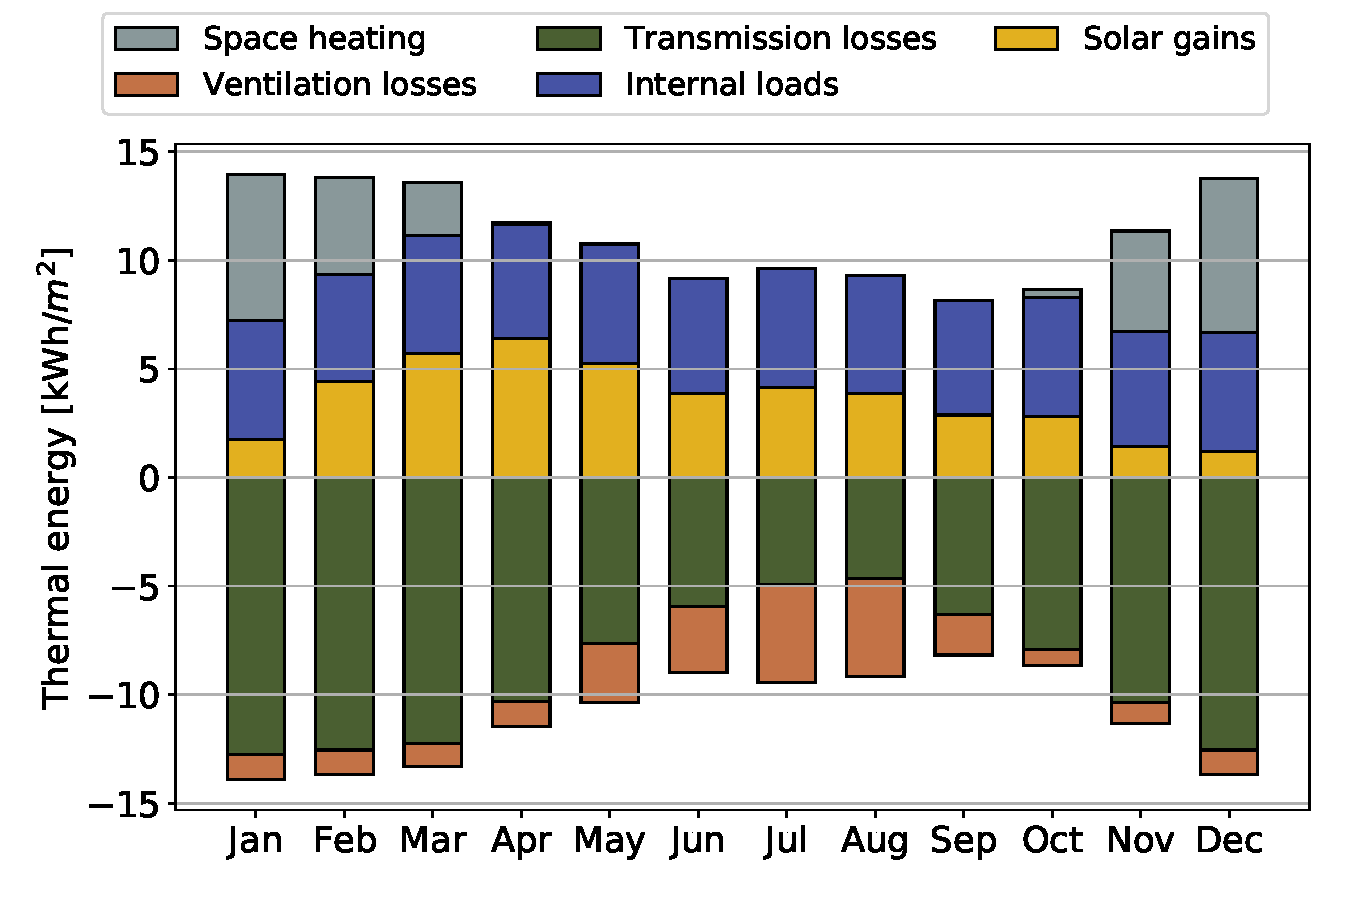
\includegraphics[scale=0.34]{img/HDU_Enbal.pdf}
%\vspace{2pt} 
\caption{Simulated energy balance of the building.}
\label{fig:HDU_Enbal}
\vspace{-5pt}  % Please use appropriate negative vspace to remove the space above/below the Table
\end{figure}

\begin{table}[H]
%\vspace{-5pt}  % Please use appropriate negative vspace to remove the space above/below the Table
\caption{Building energy performance indicators}
\label{tab:indicators}
\centering
\begin{tabular}{| c | c | c | }
  \hline
  \bf{Indicator} & \bf{kWh/$m^2a$} \\
  \hline
  Space heating energy demand & 25.9 \\
  Domestic hot water energy demand & 21.7 \\
  Electrical energy consumption & 44.0 \\
  Final energy demand & 60.8 \\
  \hline
\end{tabular}
\vspace{-5pt}   % Please use appropriate negative vspace to remove the space above/below the Table
\end{table}

%---------------------------------------------------------------------------------------
\subsection*{PV system and battery}
%---------------------------------------------------------------------------------------
The total yearly electricity demand is 3424 kWh/a, and the energy generated by the PV system is 3224 kWh/a. The HDU generates 98\% of the electricity that it consumes on an annual basis, which means that carbon neutrality in he building operation is almost reached. Figure \ref{fig:HDU_PVbal} shows the monthly energy consumed and generated. In summer months, the generation is around twice the consumption. In winter, the high consumption (mainly due to space heating) overcomes the generation. However, the average self-consumption is 83\%, meaning that this amount of the generated energy is consumed, and the rest must be taken from the grid. This confirms the ability of the energy management system to optimize the battery charging behavior in order to minimize the grid energy consumption, illlustrated in figure \ref{fig:HDU_ELbal}.\\ 

\begin{figure}[H]
\vspace{-2pt} 
\centering
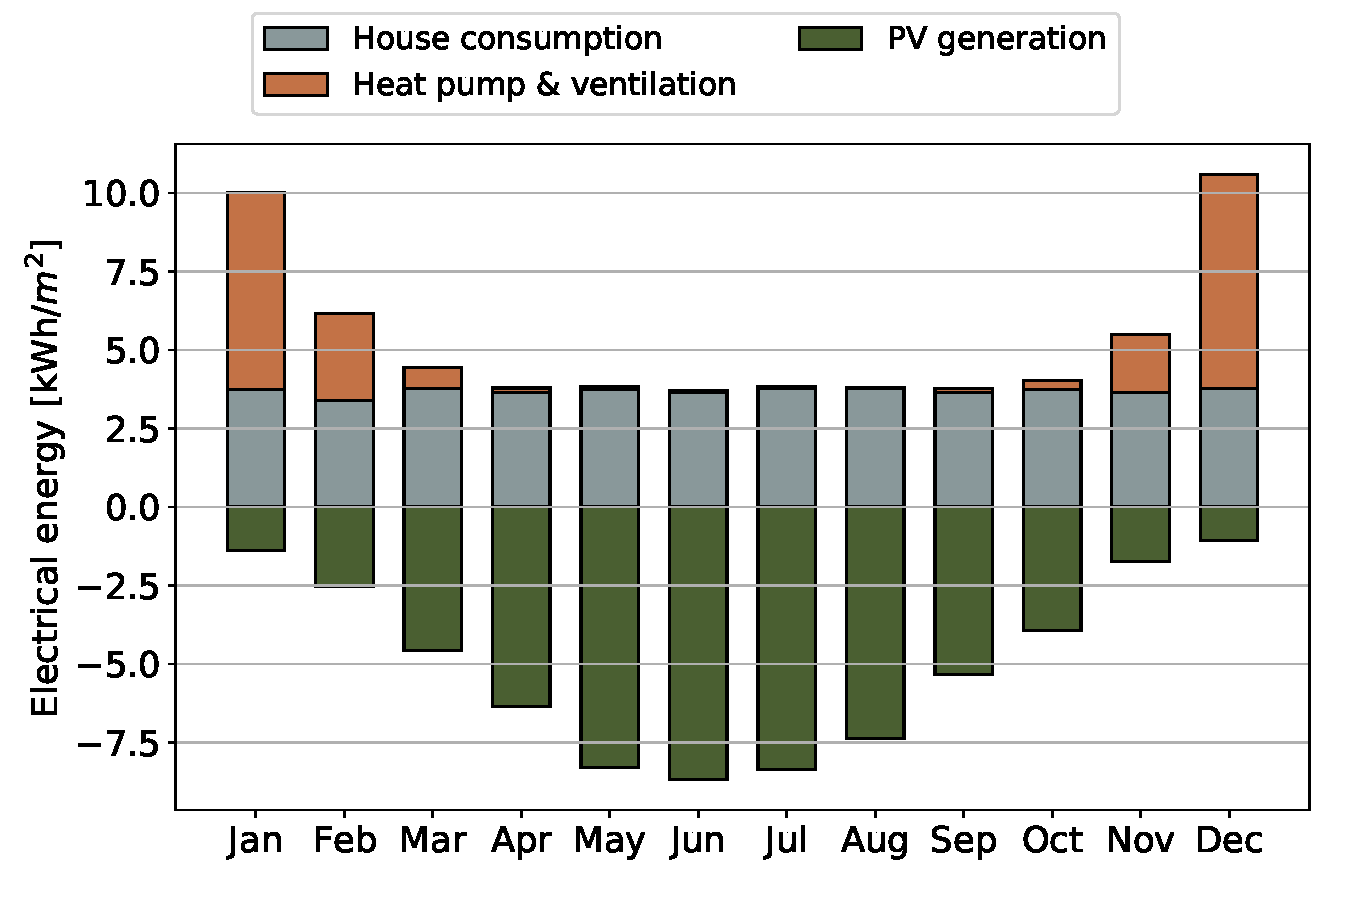
\includegraphics[scale=0.34]{img/HDU_PVbal.pdf}
\caption{Monthly energy generated and consumed.}
\label{fig:HDU_PVbal}
\end{figure}

\begin{figure}[ht]
\vspace{-5pt} 
\centering
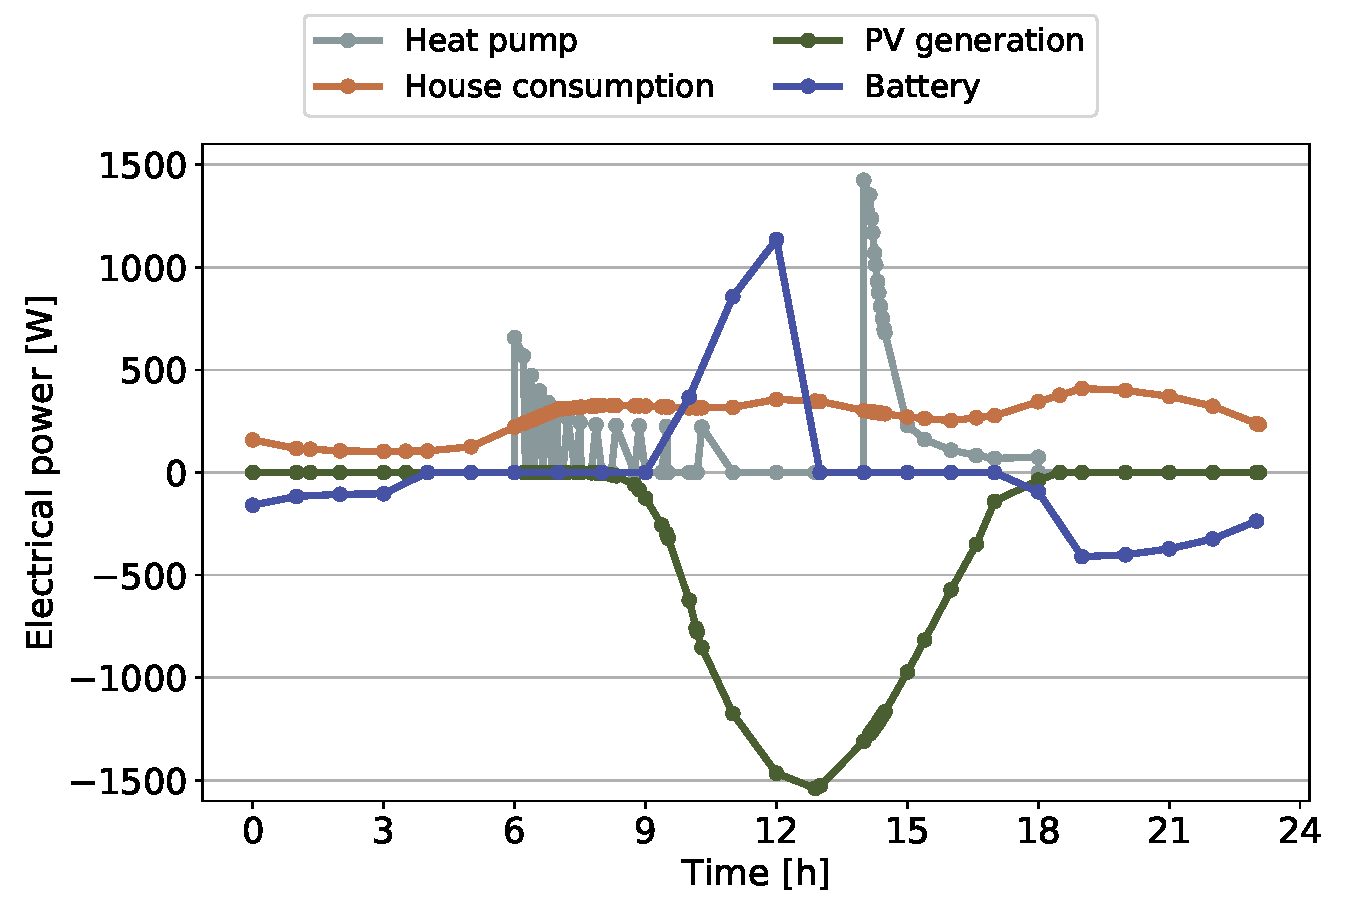
\includegraphics[scale=0.34]{img/HDU_ELbal.pdf}
\caption{Battery charging behavior on a typical winter day.}
\label{fig:HDU_ELbal}
\end{figure}

%---------------------------------------------------------------------------------------
\subsection*{Solar-assisted heat pump}
%---------------------------------------------------------------------------------------
The coupling of the heat pump and the PVT collects as its heat source was evaluated. Results show that 12 PVT collectors in parallel are an acceptable trade-off between the winter and summer optimum (28 collectors for a maximum COP of the heat pump versus 6 collectors for sufficient domestic hot water supply). The total heat delivered by the heat pump for floor heating and domestic hot water amounts to 2571 kWh. With a total electrical energy consumption of 1027 kWh/a, the heat pump has a seasonal COP of 2.51. Using the PVT collectors as single heat source for the heat pump results in a high heat pump performance when the sun shines (COP is 5.85 when the heat pump generates domestic hot water in summer). In winter, the solar radiation is lower, thus the collectors must be shut down to avoid icing on the back side, which can lead to structural damages (The manufacturer recommends not to operate the collectors when the brine temperature goes below 2°C, what was also implemented in the simulation model). In those cases, the heat comes solely from the electrical back up system. This leads to a decreased overall system efficiency and lower COP values when the outdoor temperature is below 0°C. Figure \ref{fig:HDU_HPop} shows the operation of the heat pump on a typical winter day.\\

\begin{figure}[H]
\vspace{-5pt} 
\centering
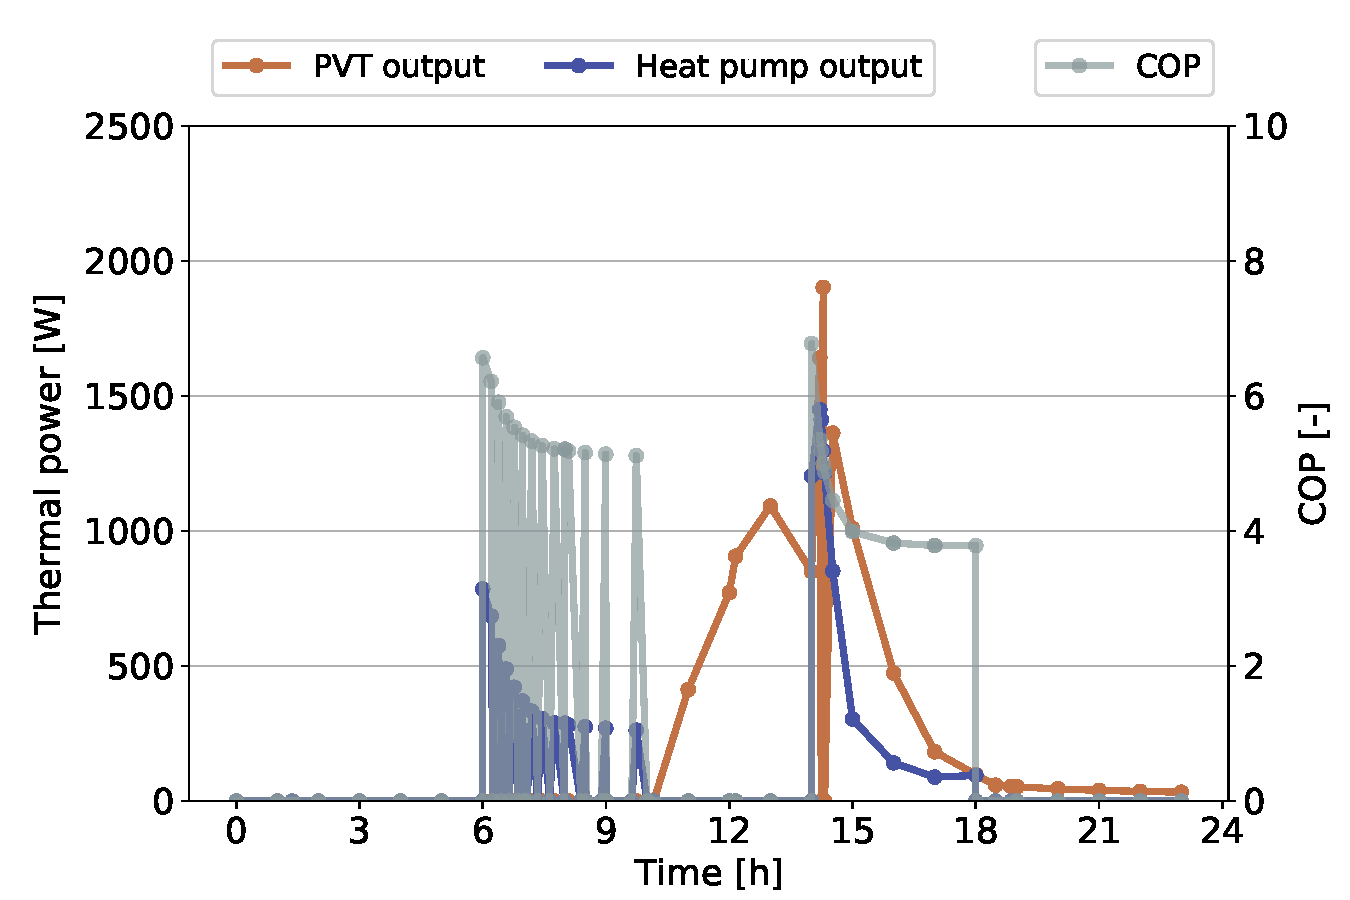
\includegraphics[scale=0.34]{img/HDU_HPop.pdf}
\caption{Heat pump behavior on a typical winter day.}
\label{fig:HDU_HPop}
\end{figure}

\begin{figure}[H]
\centering
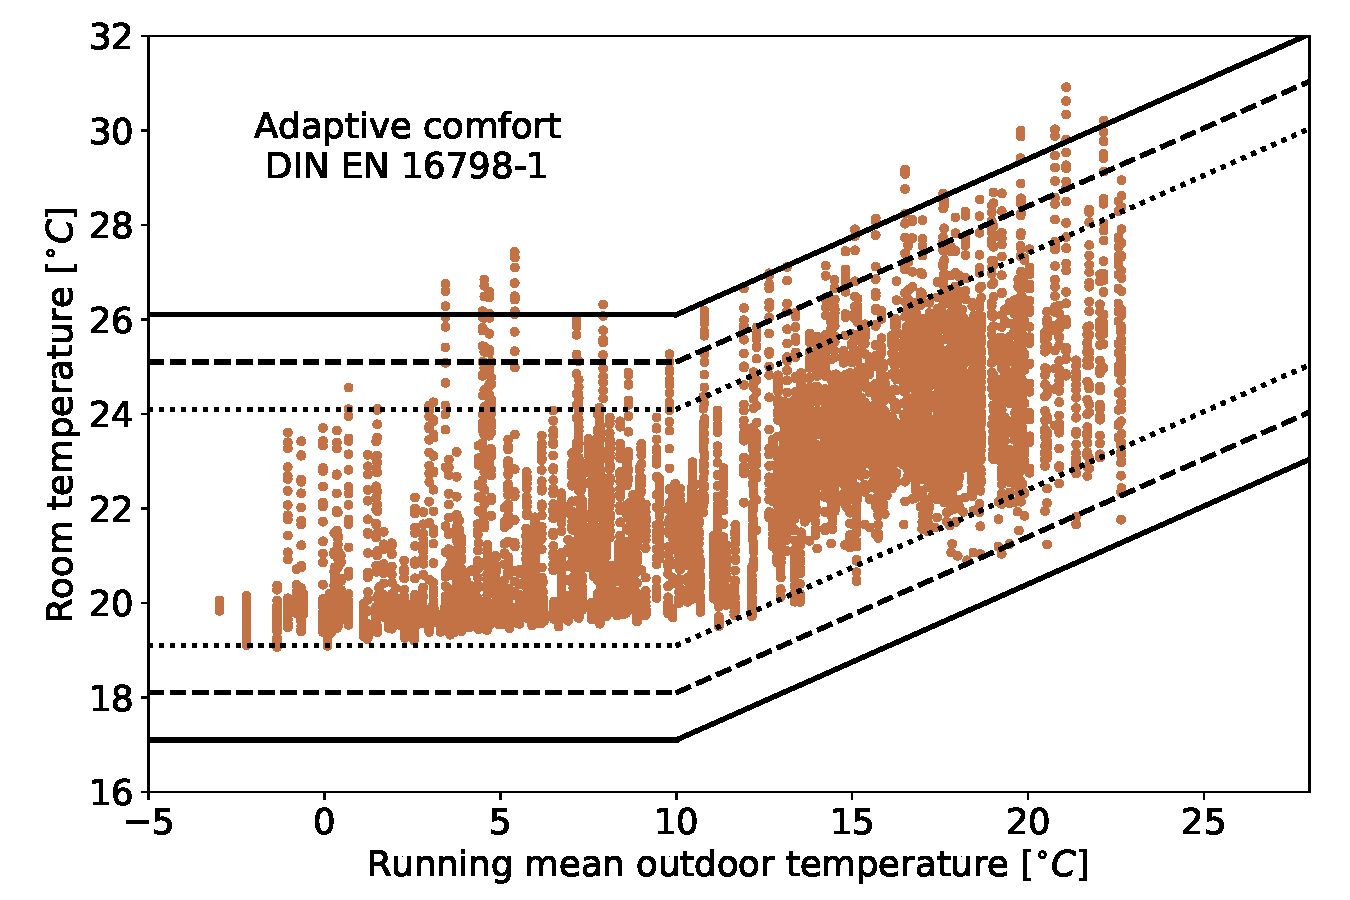
\includegraphics[scale=0.34]{img/HDU_adcomf.pdf}
\caption{Simulated indoor thermal comfort results based on the adaptive comfort model - \cite{DIN16798}.}
\label{fig:HDU_adcomf}
\end{figure}
%---------------------------------------------------------------------------------------
\subsection*{Thermal comfort}
%---------------------------------------------------------------------------------------
Comfort and well-being was among the priorities throughout the design process which results in a variety of different measures to ensure high indoor environmental quality. For effectively discharging the thermal mass by night ventilation, reasonable ventilation rates have to be achieved. Figure \ref{fig:HDU_adcomf} shows the simulated indoor temperatures as a function of the outdoor temperature running mean. Around 90\% of the time the indoor temperature is kept within the desired range of the adaptive comfort model according to \citet{DIN16798} (categories 1 and 2) for 90\% of the time. The skylights are operated automatically through the energy management system which also involves the occupants into the decision process (through push notifications in a user interface).\\ 

\vspace{-5pt} 
\begin{figure}[H]
\centering
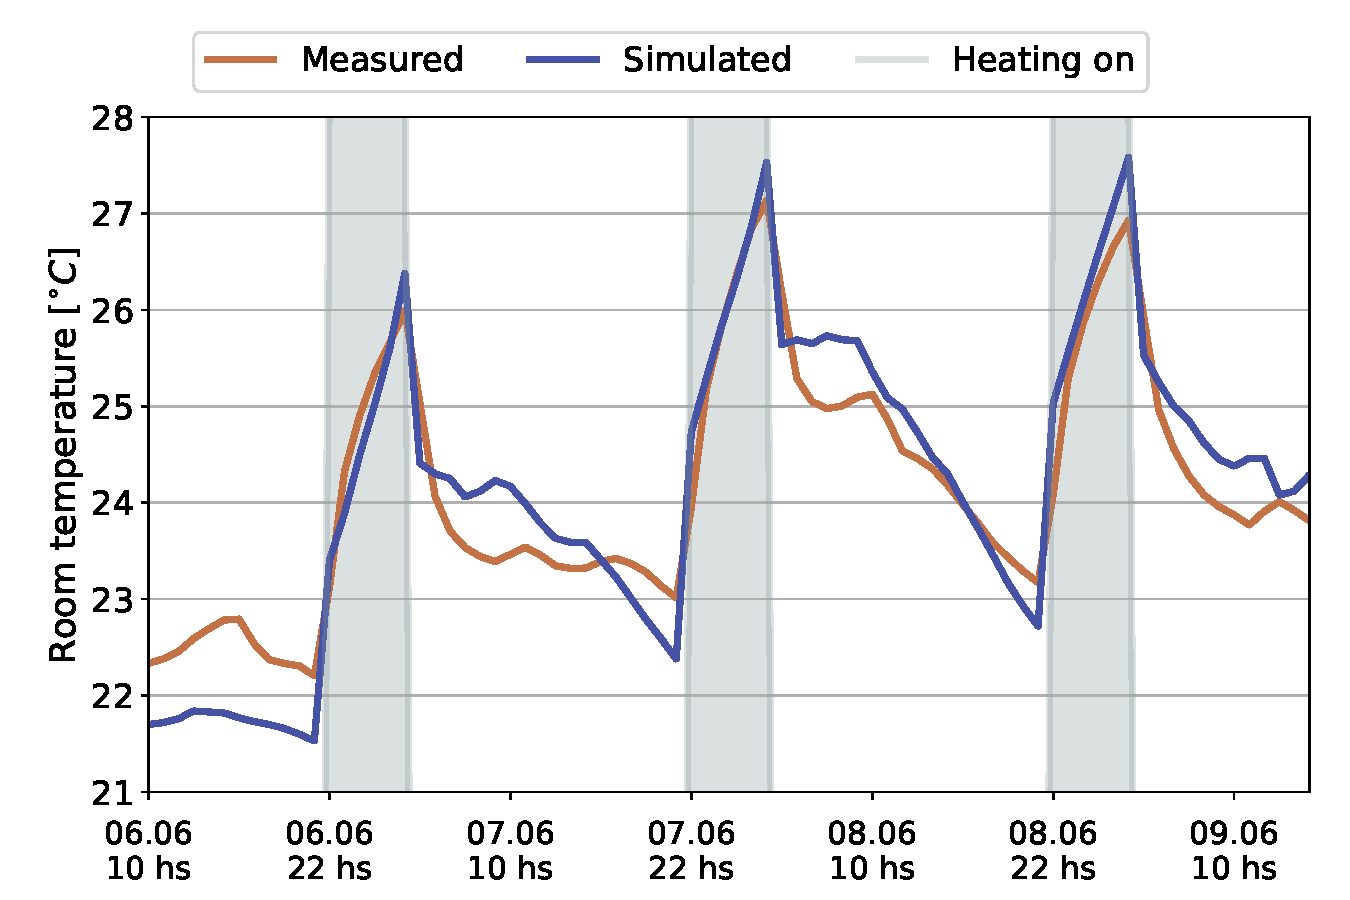
\includegraphics[scale=0.34]{img/Mess_PGC.pdf}
\caption{Measured and simulated indoor temperature during competition.}
\label{fig:Mess_PGC}
\end{figure}

During competition in Wuppertal, the Performance Gap Test took place, in which the indoor temperature of the unit was measured. The internal loads were remotely controlled in time slots (2.5 KW heater), besides having all windows and blinds closed. Figure \ref{fig:Mess_PGC} shows the comparison of the simulated and measured temperature, according to the developed building model. The agreement between both curves is high, confirming the ability of the developed model to represent the physical effects in the building. This comparison against real measurements was performed after the simulation study, therefore it confirms the validity of the results presented in this publication.  
%---------------------------------------------------------------------------------------
\section*{Conclusion}
%---------------------------------------------------------------------------------------
The paper presents a building concept realized within the Solar Decathlon Europe 21/22, which combines ambitious targets in terms of CO2 neutrality during the operation of the building unit by harvesting solar energy and using heat recovery. Besides the care about the environmental impact, occupants' well-being and comfort is of utmost importance for the building design and operation. Simulations were performed by students of different faculties (architecture, building services, mechanical engineering), complementing each others' competences and improving both their theoretical foundations and practical simulation experience. \\
The solar-based heating system was optimized by system simulation (both in terms of collector area and optimal orientation).Using the simulation model presented in this publication, team RoofKIT took decisions regarding the PVT collectors area and angle, the storage control strategies (both buffer tank and battery) and the developed controllers for the heat pump and solar water heating system. As a result, a seasonal COP of 2.51 for the heat pump was reached due to using the PVT collectors as a heat source (together with a large buffer tank and the developed controller). RoofKIT primarily uses electricity directly produced by the PVT collectors or stored in the batteries. Additional needs have to be covered by the grid but they are low due to the energy management system optimizing the self-consumption. Balancing electricity demand from the grid and surplus electricity fed into the grid, the building can be operated almost carbon neutral. \\
Thermal comfort in winter is achieved by high-level insulation of the building envelope, ventilation heat recovery and a radiant heating system. Simulations showed that indoor temperatures are within the boundaries of the adaptive comfort model most of the time. In summer, passive cooling guarantees a comfortable indoor environment.\\
Besides the work here presented, other simulations were carried out that supported the decision-making process. Daylighting simulations were used to determine the window area and positioning. CFD simulations were performed to study the influence of night ventilation in local thermal comfort and draft risk. Regarding the building envelope, simulation using SimRoom (\citeyear{SimRoom2022}) were carried out to optimize the insulation thickness and thermal mass.\\
The RoofKIT team wants to set an example for simulation-based future building design. An integrated design strategy yields to utilize all available possibilities with regard to materials, construction and renewable energy supply in order to set a sign for high quality architecture – also as a symbiosis of 'old' and 'new'. Building simulation and optimization was used as one of the main decision-making tools for building design, highlighting its relevance to be included in an educational context to a wider extent.\\

%---------------------------------------------------------------------------------------
\section*{Acknowledgment}
%---------------------------------------------------------------------------------------
The project is supported by funding from the German Federal Ministry for Economic Affairs and Climate Action (BMWK), the Karlsruhe Institute of Technology (KIT), the Baden-Württemberg Ministry of Food, Rural Areas and Consumer Protection, as well as cash and in-kind contributions from numerous sponsors.\\
%---------------------------------------------------------------------------------------
%References
\bibliographystyle{BSO2022}
\bibliography{references}

\end{document}
